\documentclass{article}
\usepackage{pdfpages}
\usepackage{listings}
\usepackage{amsfonts}
\usepackage[T1]{fontenc}
\usepackage{xcolor}
\usepackage{placeins}
\usepackage{float}
\usepackage{underscore}
\usepackage[bookmarks=true]{hyperref}
\usepackage[utf8]{inputenc}
\usepackage[margin=0.5in]{geometry}
\usepackage{graphicx}
\usepackage{subfigure}
\usepackage[english]{babel}
\hypersetup{
	bookmarks=false,    % show bookmarks bar?
%	pdftitle={Text Analytics Tutorial 5},    % title
	pdfauthor={Adam-Ryan},                     % author
	pdfsubject={TeX and LaTeX},                        % subject of the document
	pdfkeywords={TeX, LaTeX, graphics, images}, % list of keywords
	colorlinks=true,       % false: boxed links; true: colored links
	linkcolor=blue,       % color of internal links
	citecolor=black,       % color of links to bibliography
	filecolor=black,        % color of file links
	urlcolor=blue,        % color of external links
	linktoc=page            % only page is linked
}%
\def\myversion{1 }
\date{}
%\title
\usepackage{hyperref}
\begin{document}
	
\section{Exercise 1}
This is the answer to question 1.
\begin{enumerate}
	
	\item k-NN is a classification algorithm. Broadly speaking, the algorithm works by taking a Metric Space $(X,d)$, where X is the set of all datapoints (X split into seen and unseen datasets) and $d$ is commonly taken as $d_E$ and a fixed value $k \ge 0$ with $k \in \mathbb{N}$. For a new unseen data point which you wish to classify, the distance between this point and all seen points is calculated. The subset of the k closest points to the new unseen data points are taken. The new datapoint is then assigned the class which most frequently occurs in the subset. In the instance that there is an equal distance or equal number of points, there are multiple ways of dealing with this in the implementation of k-NN, including choosing the 'first best' class, 'last best' class, or previous assignment, but typically this is an implementation detail and in practice is not typically important. As $k \rightarrow \infty$, the time and space requirements grow; choosing the value of $k$ which maximises performance is a key element in the usage of k-NN.
	
	\item n-Fold Cross-validation is a method of training a model with a goal of decreasing bias when limited data is available. The dataset is partitioned into $n$ subsets. $n-1$ subsets are taken as training data, and the remaining subset is taken as the test data. The model performance is noted, and then the process is repeated such that every subset has been used as the test data once and only once. The model is then assessed by taking the mean (or other comparative measures depending on the precise situation) of all results. It's worth noting that this implementation of n-Fold Cross-validation is not appropriate to time series data, and for data where time plays an important factor rolling cross-validation must instead be used, however this is not relevant to this particular question over the iris dataset.
	
	\item For the question I implement SKLearn's nearest neighbour classifier with the Euclidean distance. For the following values:\\
	\\
	split\_array = [0.1,0.28,0.46,0.64,0.82] with a k-value of 12 (the square root of the number of instances)
	\\
	\\
	k\_array=[2, 4, 6, 8, 10, 12, 14, 16, 18, 20, 22] with a test size of 36\% of the data and using 5-Fold Cross Validation\\
	\\
	I generate the following plots:
		\begin{figure}[h!]
		\centering
		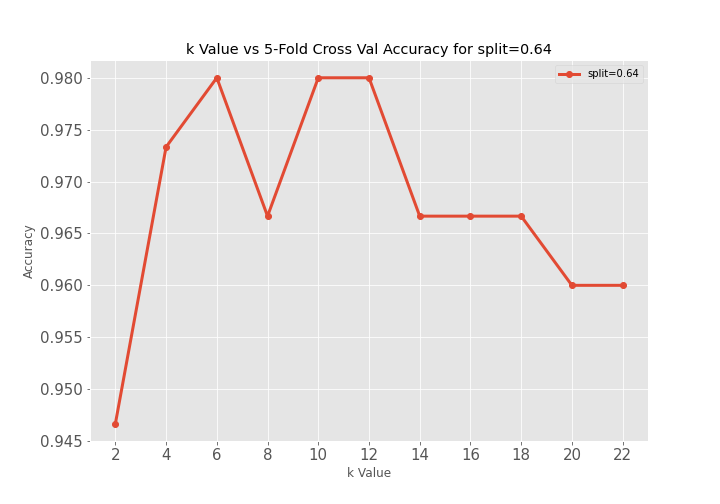
\includegraphics[width=0.4\linewidth]{k_vs_accuracy.png}\
		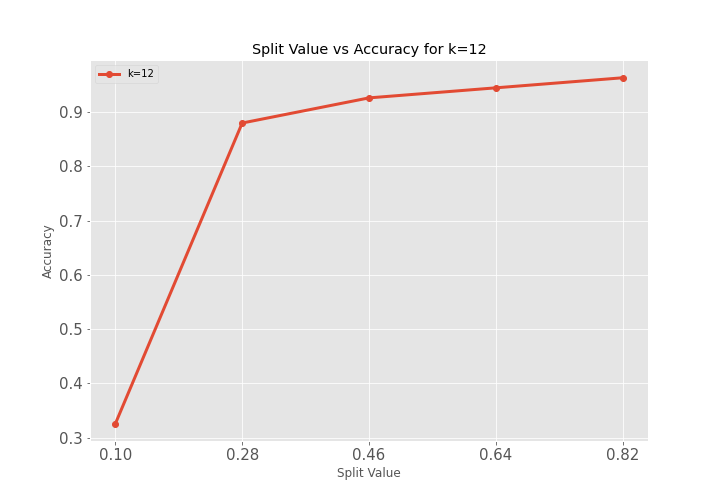
\includegraphics[width=0.4\linewidth]{split_vs_accuracy.png}
		\caption{Question 1}\label{tfidf}
	\end{figure}
\\
For each run of the process I generate a report using sklearn's metrics and cross\_val\_score (with criteria set as accuracy). which I subsequently use to generate these plots. A sample in running through the k\_array when k=16 is listed below:
\newpage
\begin{verbatim}
	-
	16-Nearest Neighbours:
	-
	Total Time to Classify: 0.0021959580008115154
	----DETAIL----
	
	
	Accuracy: 
	
	0.9074074074074074
	
	
	Confusion matrix: 
	
	array([[16,  0,  0],
	[ 0, 17,  4],
	[ 0,  1, 16]])
	
	
	Classification report:
	
	{'Iris-setosa': {'precision': 1.0,
			'recall': 1.0,
			'f1-score': 1.0,
			'support': 16},
		'Iris-versicolor': {'precision': 0.9444444444444444,
			'recall': 0.8095238095238095,
			'f1-score': 0.8717948717948718,
			'support': 21},
		'Iris-virginica': {'precision': 0.8,
			'recall': 0.9411764705882353,
			'f1-score': 0.8648648648648648,
			'support': 17},
		'accuracy': 0.9074074074074074,
		'macro avg': {'precision': 0.9148148148148149,
			'recall': 0.9169000933706816,
			'f1-score': 0.9122199122199123,
			'support': 54},
		'weighted avg': {'precision': 0.9154320987654321,
			'recall': 0.9074074074074074,
			'f1-score': 0.9075999075999076,
			'support': 54}}
		
	5-fold: [0.93333333,  1.         ,0.93333333, 0.96666667 1.       ]
	
	Mean Accuracy score over 5 folds: 
	0.9830751292817533
	
	Stddev Accuracy score over 5 folds: 
	0.015164328350789515
\end{verbatim}

\newpage
\item[k-Value] We see that the accuracy rises as k increases up to 6, with a slight dip when it achieves a value of 8, before returning to its peak for 10 and 12 and the gradually declining as the number of neighbours increases from there. For the iris dataset we see that a value around k=6 is likely to be optimal. A key reason for choosing a small value of k is that if k exceeds the number of test data the provided function will return an error as the number of neighbours to check will exceed the total size of the dataset, which is why I looked up to a range of 22. 

\item[split-Value] We see that as the size of the training dataset increases, the accuracy of our model increases. At split=0.28 we achieve approximately 90\% accuracy and gain only smaller gains from there. As I was using an explicit test size, using cross-validation in this instance does not make sense. As such the accuracy which is plotted is the accuracy of a single trained model on data which is randomly split according to the split size.

\end{enumerate}

\section{Exercise 2}
This is the answer to question 2.
\begin{enumerate}
	
	\item Naive Bayes is a classifier based on applying Bayes Theorem with an indepence assumption amongst all features. Broadly speaking it works by calculating the prior probability for each class, finding the likelihood probability for each class, calculating the posterior probability for each class, and then identifying which class has the highest probability and assigning that class to the datapoint. 
	
	\item I add a new feature which looks at the first letter of the name instead of the last, and also a feature which looks at the first and last letter of the name. These features are defined as:
	\begin{verbatim}
		  def last_letter(word):
			return {'last_letter': word[-1]}
		
		def first_letter(word):
			return {'first_letter': word[0]}
		
		def first_last_letter(word):
			return {'first_last_letter': word[0] + word[-1]}
	\end{verbatim}
\noindent Adding in these features results in an accuracy of 0.79 for the last letter feature, 0.7468 for the first and last letter feature, and 0.658 for the first letter. 
\item This shows us that over the test dataset, the last letter results in a stronger degree of classification than the first letter or a combination of first and last letter. For example, we see that 'k','a','f', 'p', and 'v' have a signifivant power as last letters in predicting gender, while the first letter 'W','Q','U','X', and 'K' are the most informative first letters; however, none of these first letters are as informative as the last letters. In the first and last letter set, we see there are certain combinations of first and last letters which are particularly informative, however as the overall accuracy is lower one would surmise that this trails off. Certain combinations of first and last letter may be relatively unique within the dataset resulting in poor classification results for these and resulting in an overall lower accuracy; this is sensible as the possible combinations of first and last letters are $26^2$ which would require a substantial training set to ensure all combinations are seen at least once (but ideally multiple examples would be wanted for each combination). In addition, these classification tools are challenged with gender-neutral names.

\item Exlicitly, we see the following examples are classified differently between first letter, last letter, and first and last letter; in our examples there are no clear instances of names which are right in the first letter case but not in the last letter case:
\begin{verbatim}
	Example	| Last | First | FirstLast
	Barry | Female | Female | Female - Wrong in ALL cases.
	Adam | Male | Female | Male - Wrong in FIRST case.
	Hassan | Male | Male | Male - Correct in ALL cases
\end{verbatim}

\item A sample run of the program is listed below:
	\begin{verbatim}
		-----
		LAST LETTER     
		-----     
		
		Mark is: male
		Precilla is: female
		Adam is: male
		Barry is: female
		Sean is: male
		Peter is: male
		Hassan is: male
		
		
		Most Informative Features
		last_letter = 'k'              male : female =     45.1 : 1.0
		last_letter = 'a'            female : male   =     34.2 : 1.0
		last_letter = 'f'              male : female =     17.3 : 1.0
		last_letter = 'p'              male : female =     11.9 : 1.0
		last_letter = 'v'              male : female =     10.5 : 1.0
		
		Classifier accuracy: 
		
		0.79
		
		-----
		FIRST LETTER     
		-----     
		
		Mark is: female
		Precilla is: female
		Adam is: female
		Barry is: female
		Sean is: female
		Peter is: female
		Hassan is: male
		
		
		Most Informative Features
		first_letter = 'W'              male : female =      4.6 : 1.0
		first_letter = 'Q'              male : female =      2.9 : 1.0
		first_letter = 'U'              male : female =      2.4 : 1.0
		first_letter = 'X'              male : female =      2.3 : 1.0
		first_letter = 'K'            female : male   =      2.2 : 1.0
		
		Classifier accuracy: 
		
		0.658
		
		-----
		FIRST AND LAST LETTER     
		-----     
		
		Mark is: male
		Precilla is: female
		Adam is: male
		Barry is: female
		Sean is: male
		Peter is: male
		Hassan is: male
		
		
		Most Informative Features
		first_last_letter = 'Ca'           female : male   =     54.8 : 1.0
		first_last_letter = 'Da'           female : male   =     40.4 : 1.0
		first_last_letter = 'Ma'           female : male   =     38.4 : 1.0
		first_last_letter = 'Ra'           female : male   =     38.3 : 1.0
		first_last_letter = 'Hn'             male : female =     33.8 : 1.0
		
		
		Classifier accuracy: 
		
		0.748
	\end{verbatim}
	
\end{enumerate}


\end{document}
